\section{Presentation Logic Layer}

%What pages will be present in your project? briefly indicate how your web site will be organized
There will be present approximately 10 pages. The default one will be a page showing all the past and active tournaments, that every user can check even if not logged in. A page for the login and the sign up. Once logged in, the user will be able to see also the past and active tournaments that he created. Finally, there will be the pages dedicated to displaying the information and the ones dedicated for the creation of the teams and the tournaments and for the updating of the matches.

Below are some examples of pages implementing the functionalities described before.

\begin{itemize}
    \item \textbf{Homepage:} it displays both past and active tournaments even if the user is not logged in. By clicking on a past tournament all the details are shown (results, both table ecc.); by clicking on an active one it is displayed the same thing but in realt time (to be updated). In the top right corner there is a button that allows the login for the user.\\\\
    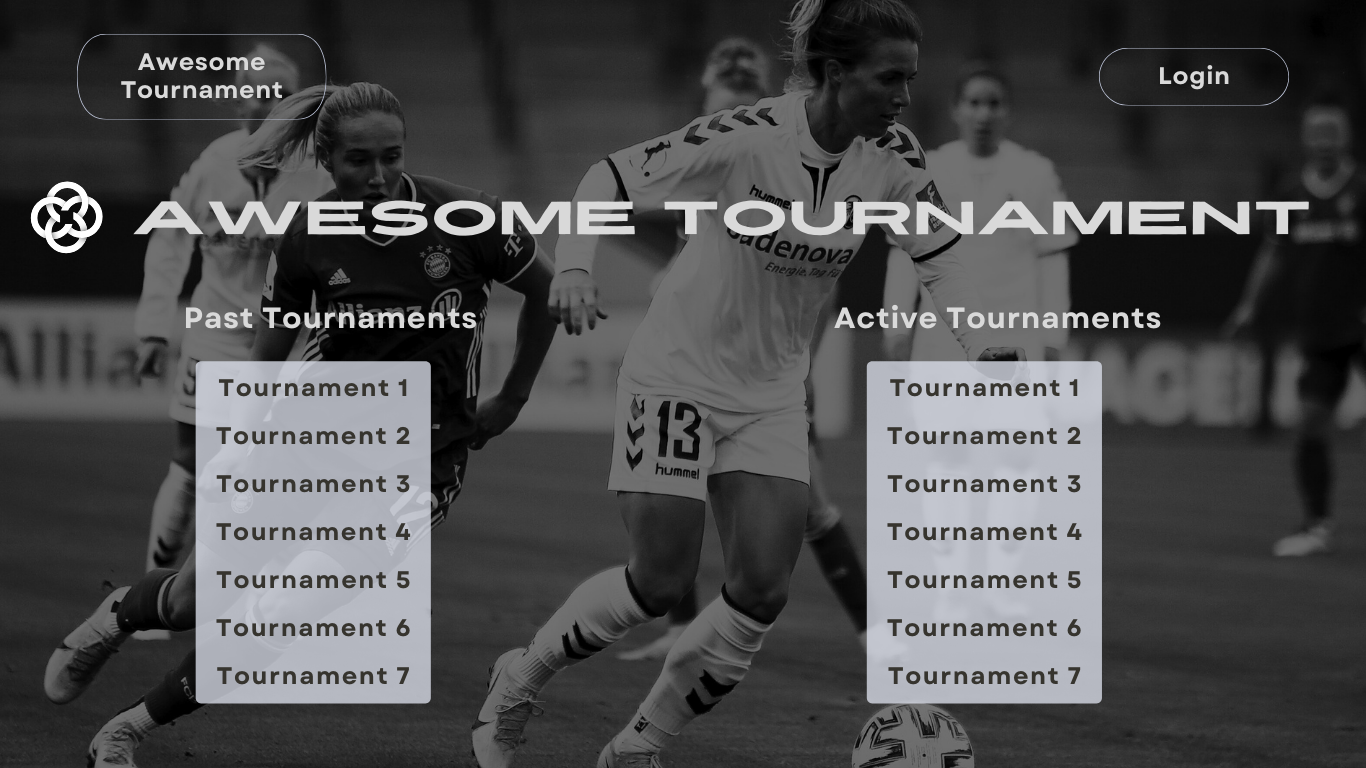
\includegraphics[scale = 0.36]{sections/homepage.png}

    \item \textbf{Login in page:} it is requested to provide a valid email and a secure password. By clicking on "Sign up" the user can register on the site.\\\\
    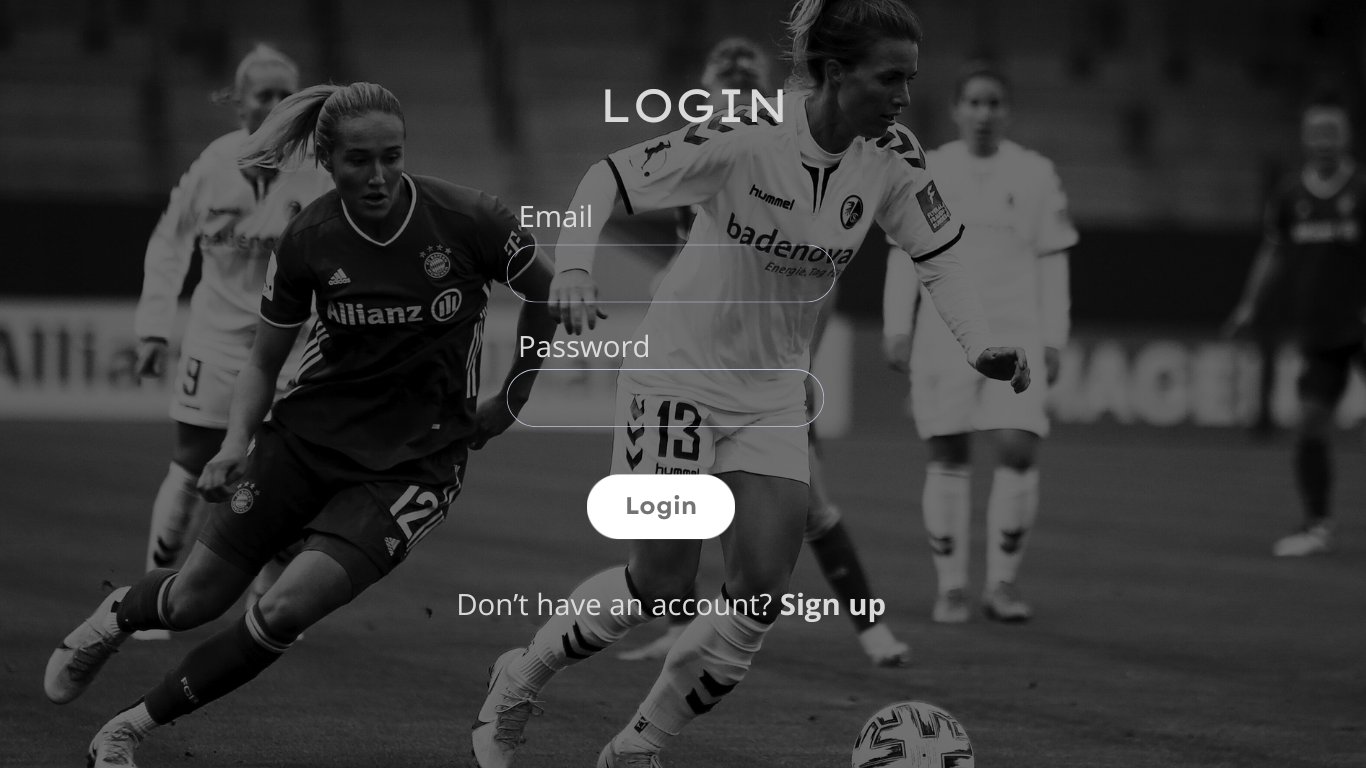
\includegraphics[scale = 0.36]{sections/login.png}

    \item \textbf{Homepage after login:} after the login all the past and active tournaments created by the user are displayed. From here the user can start the process to create a new tournament.\\\\
    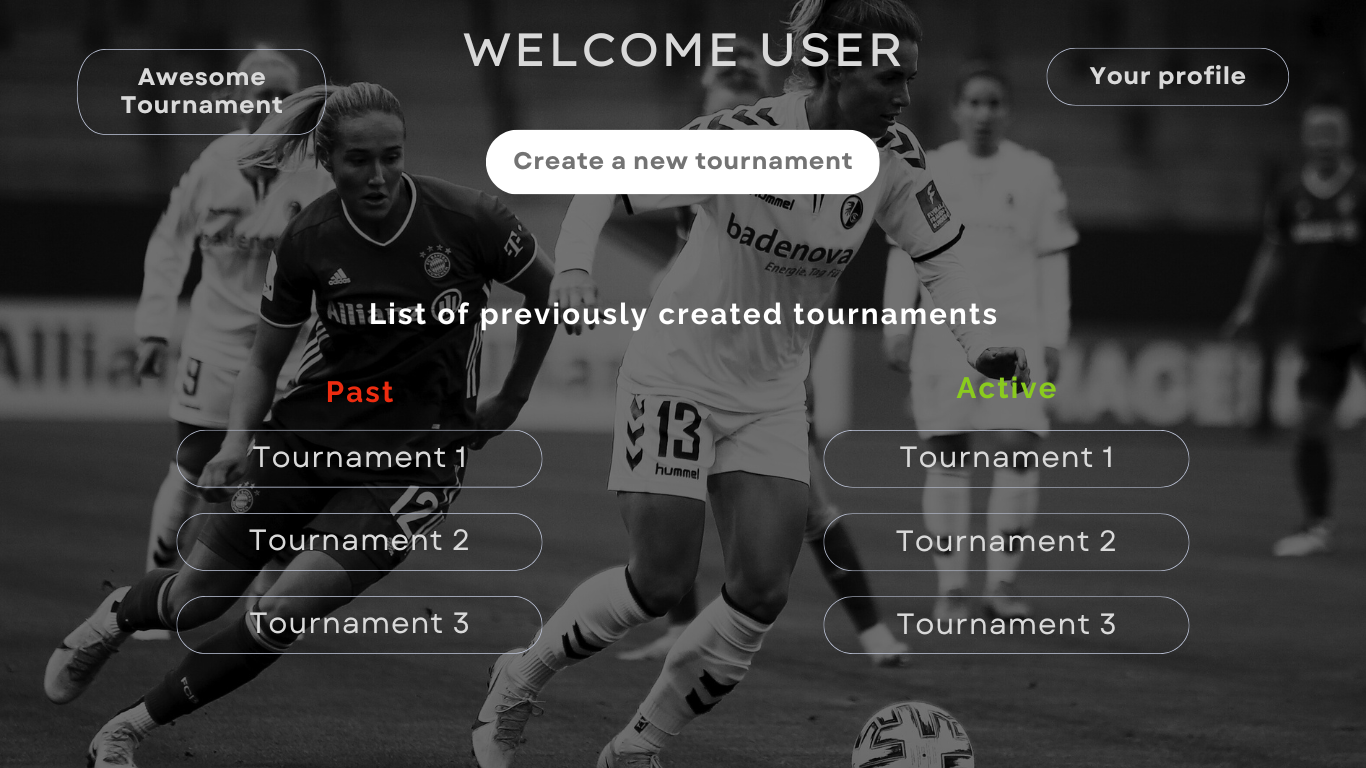
\includegraphics[scale = 0.4]{sections/homepagelogin.png}

    \item \textbf{Page of a tournament:} the page displays the infos about a tournament. The user can decide what to check from the three button (Results, Table and Top scorer). It is also possible to choose the matchday to check. For the admin of the tournament and the creator of that team it is also possible to manage the team.\\\\
    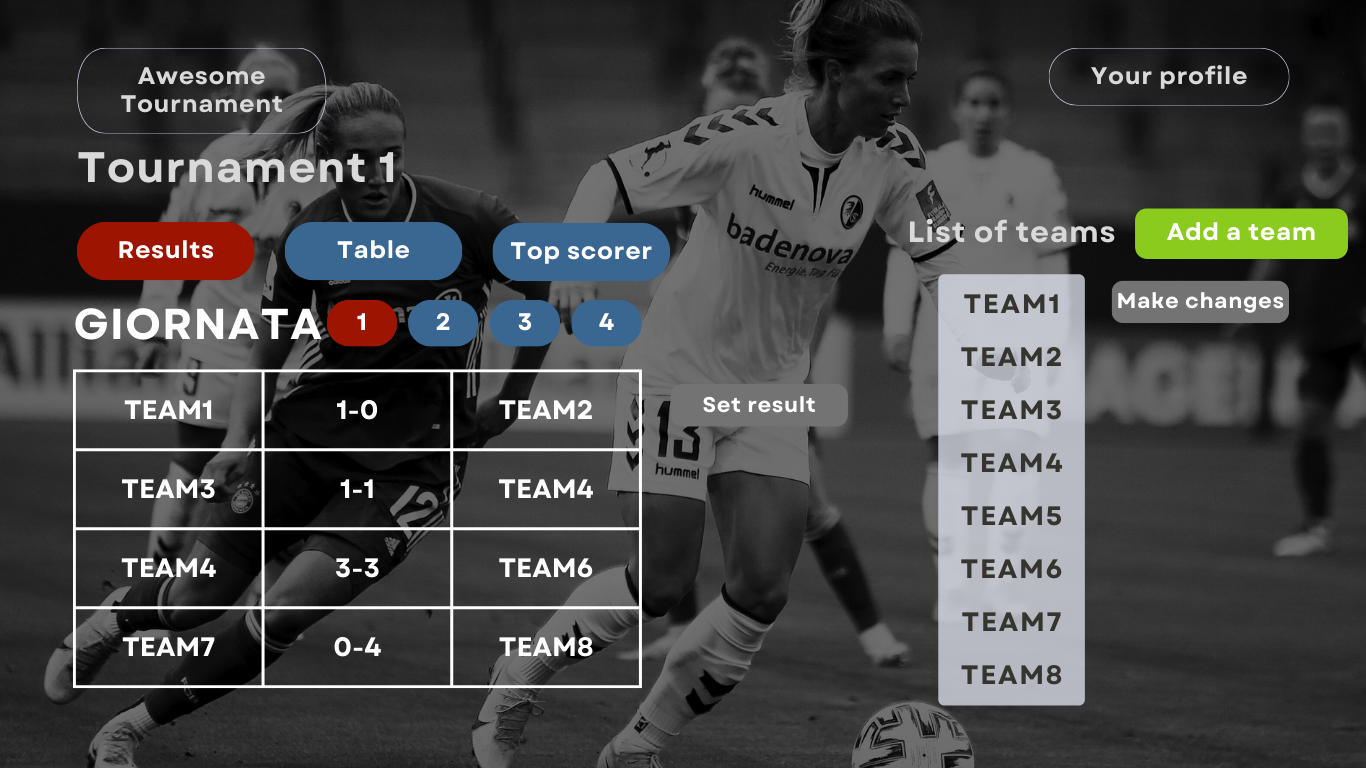
\includegraphics[scale = 0.4]{sections/webpage.png}

\newpage

    \item \textbf{Page of a specific match:} the page displaying the infos about a specific match of a tournament. Only the admin of the tournament is allowed to fill in the events for a match by clicking on "update result and scorers".\\\\
    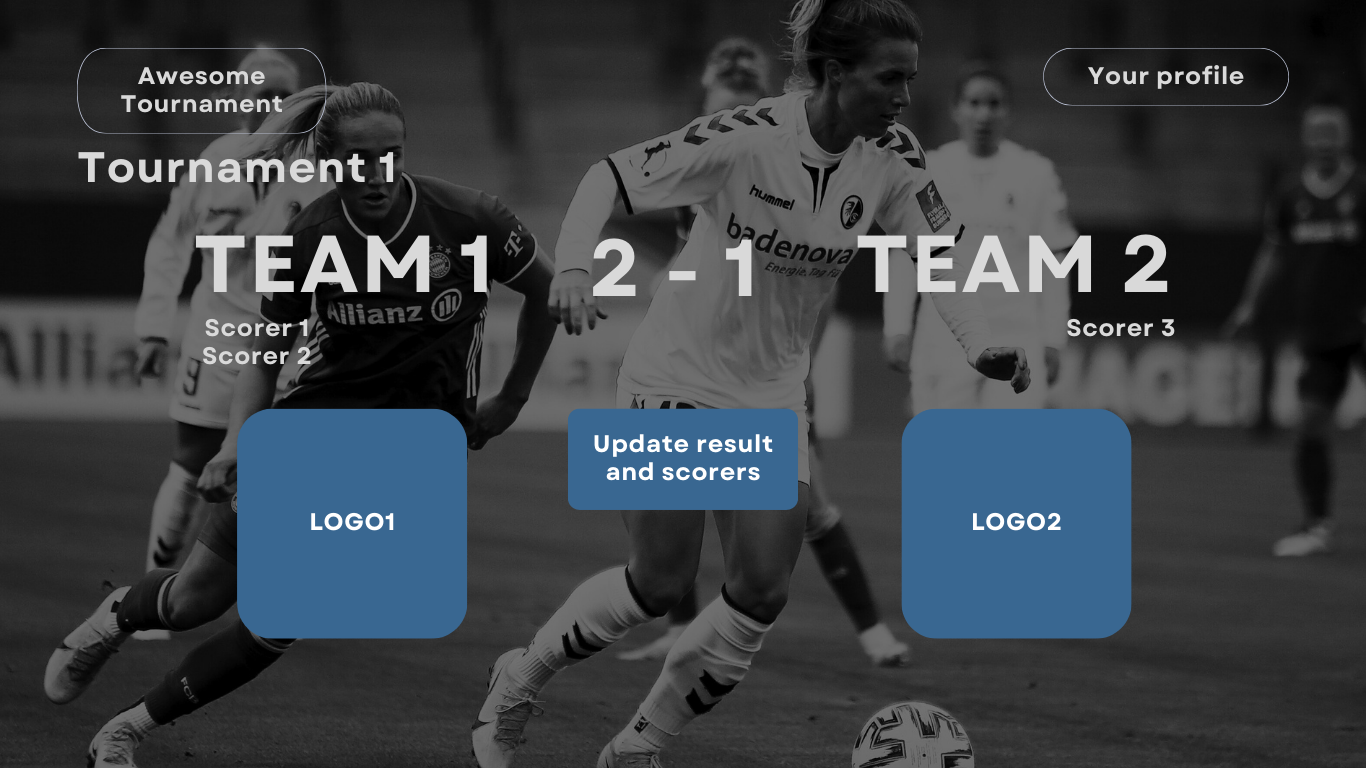
\includegraphics[scale = 0.4]{sections/match.png}

    \item \textbf{Process of creating a tournament:} the image below display the process of creating a tournament. Only the last required info are displayed, like the starting date, the deadline and the logo.\\\\
    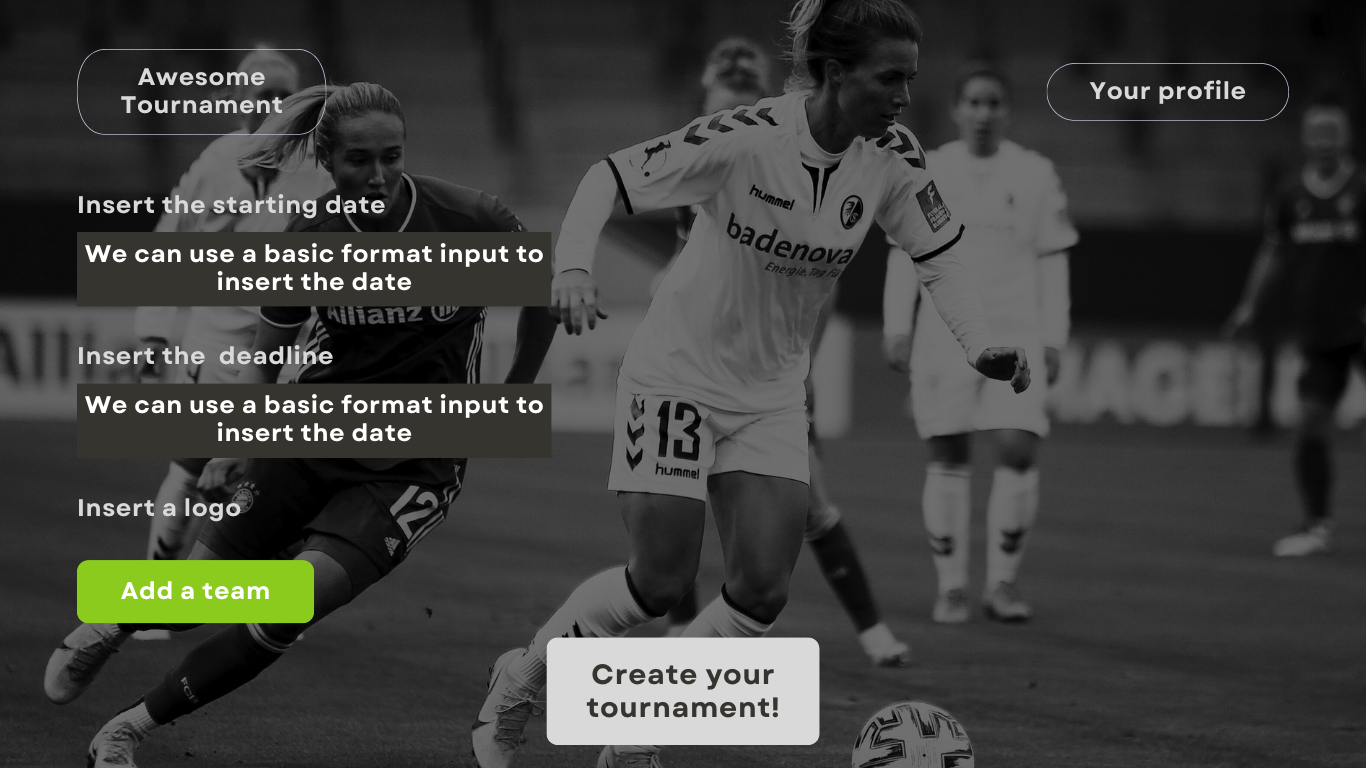
\includegraphics[scale = 0.4]{sections/createtour.png}
\end{itemize}